\documentclass[a4paper,10pt,twocolumn,twoside]{article}
\usepackage{fullpage}
\usepackage{graphicx}
\usepackage{pgfplots}
\usepackage{pgfplotstable}
\usepackage{filecontents}
\usepackage{booktabs}
\usepackage{tabularx}
\usepackage{tikz}
\usepackage{listings}
\usepackage{authblk}
\usepackage{caption}
\usepackage{mathtools}
\usepackage{underscore}
\usepackage{url}

\usetikzlibrary{patterns,shapes,positioning,calc}

\lstset{language=C, basicstyle=\ttfamily\small, columns=flexible}

\pgfplotsset{compat=1.8}

\author{Lars Kirkholt Melhus}
\author{Rune Erlend Jensen}
\affil{Norwegian University of Science and Technology}
\title{Measurement Bias from Address Aliasing}
\date{} % This is a timeless piece

% Pretty printing of performance counter names
\newcommand{\perfctr}[1] {
  \small{\uppercase{#1}}
}

\begin{document}

\twocolumn[
  \begin{@twocolumnfalse}
    \maketitle
    \begin{abstract} % Should be 150 -- 200 words max
    % Motivation -- Problem statement -- Approach -- Results -- Conclusions

    In this paper we identify the underlying mechanics resulting in measurement bias on modern Intel microarchtectures. 
    The magnitude of this performance bias has been shown to be significant, and can be as high as a factor two.
    
    We analyze a small program that was presented as a curiosity in previous work on \emph{measurement bias};
    Code that for unexplained reasons performs significantly worse than average for certain configurations of system environment variables.

    Using hardware performance counters, we identify a strong correlation with resource stalls, ultimately caused by address aliasing events.
    The CPU uses an optimistic strategy when issuing operations out of order.
    Only the last 12 address bits are compared to determine if there was a conflict, sometimes resulting in performance penalties from false dependencies.

    We show how address aliasing can cause measurement bias for two particular external properties; environment variable size, and dynamically linked heap allocation libraries.
    Performance penalties from unfavorable memory address allocations can be more than double the cycle count, even for real world applications.
    Furthermore, the dynamic memory allocation pattern for common libraries like libc tends to give worst case performance by default for large allocations.

    \end{abstract}
    \bigskip
        
  \end{@twocolumnfalse}
]


\section{Introduction}
% - Measurement bias in systems research
%   - What is measurement bias
%     - fundamentally anything external
%     - Room temperature
%   - Studied before
%     - External properties that affect memory layout
%       - link order (not really)
%       - env size
%   - Has been shown to be significant and commonplace
%     - But difficult to deal with
%     - Need to apply statistical methods to experiments
%       - randomization of experimental setups
% - Want to look at flipside: understand what why bias occurs
%   - Use for optimization
%   - Find interesting cases
%   - Known causes: cache alignment, ignore.
% - Analysis: 
%   - Use known example that exhibit bias
%   - Find lesser known source in address aliasing
% - Results:
%   - Applicable general knowledge about Intel architecture
%   - Useful for optimization
%   - Libraries and compilers fail to account for it in reality.

How fast does an algorithm run?
Is program A faster than program B on \emph{my} machine?
These types of questions are, perhaps surprisingly, not always trivial to answer.
The usual approach to quantify performance is to simply measure some metric, such as the wall time or number of cycles executed.
However, performance is not just a function of the collection of instructions in an executable, but also dependent on various \emph{external} factors.

In other fields of science, accounting for sampling bias is well understood.
Trying to determine the political opinion of a country just by sampling a narrow geographical area will probably not be very accurate.
The same concept applies for software; measuring a metric once is analogous to sampling only a tiny geographical area in the set of possible system configurations.

There are many external variables that has the potential to affect system performance.
In particular, anything which can offset memory addresses of code or data at run-time can be significant.
Memory accesses interacts with low level hardware buffers, which can heavily favor certain memory layouts over others.
Consequentially, any environmental factor that can alter memory layout has a potential performance impact.
Failing to account for these effects lead to \emph{measurement bias}. 

% This is basically former background section
Measurement bias has been shown to be commonplace and significant in real applications~\cite{Mytkowicz:2008:OE&MB, Mytkowicz:2009:WrongData, Mytkowicz:2008:Easy}.
Previous work looks at environmental factors such as the size of Unix environment variables, which affects memory by offsetting the initial position of stack.
Because of the complexity of modern hardware, it is often impossible to predict exactly how seemingly innocuous things such as environment variables ultimately affect program execution.
While effects of bias has been shown to be commonplace and significant, they are unpredictable and difficult to deal with.
Without an accurate understanding of the underlying memory interactions, the best one can do to accurately assess performance is generally to average over a large sample set of execution contexts.
Previous work focuses mostly of how to account for bias by proper sampling, using randomization of execution contexts and statistical methods. % Cite is basically the same as above, all three are about the same -- difficult to split. 

Our approach is instead to try to understand some of the underlying reasons to why bias can occur, in an attempt to utilize this knowlege for potential optimization. % Could have a sentence with cite of Blind Optimization.
Usually, the root explanation will be that different memory layouts interact with various hardware buffers.
Certain mechanisms such as cache contention or branch misprediction are already well understood, thus we are looking for the more esoteric processor features.
Analyzing a program that exhibits strong bias from environment size, collecting about 200 events using hardware performance counters, we find strong correlation with resource stalls from \emph{address aliasing}.
Aliasing is an artifact of a much lesser known, presumably Intel specific, optimization on the out-of-order execution pipeline.
In short, the CPU uses a heuristic for determining whether memory loads are dependent on previous writes, comparing only the last 12 virtual address bits.
False dependencies incur performance penalties, and we show how this can explain many common cases of measurement bias.

In addition to environment variables, we look at dynamic heap allocation libraries as an external factor that can trigger (or amplify) bias resulting from address aliasing.
We find that most libraries tend to produce worst case behavior by default with respect to aliasing, caused by favoring page alignment for large allocations.
The cost of address aliasing can be significant, exemplified with a simple program yielding more than 50~\% speedup based on heap address alignment alone.
% [This next part might be added to the abstract in some form:] 
Fortunately, with an understanding of the underlying mechanisms, measurement bias from address aliasing can often be quite accurately predicted.
For some applications it might even make sense for programmers to actively take aliasing into account for architecture specific optimization, as neither compilers nor heap allocators seem to handle it well.



\subsection{Methodology}
% - Goal: Produce empirical data showing what causes bias
% - Two pitfalls:
%  - Observer effect
%  - Measurement bias
% - Hardware performance counters
%   - MSR, architecture specific
%   - Closest thing to the CPU
%   - Use perf-stat
%   - Control cache metrics
% - Best practices for controlled experimental setup
%   - No ASLR, what it is
%   - No hyperthreading, disable frequency scaling.
% - Experimental setup
%  - Intel haswell architecture
%    - Restrict to a single cpu to limit scope

In order to understand bias behavior it is important to be able to do precise measurements.
Besides measurement bias in itself, one must also consider \emph{observer effect}.
Any kind of instrumentation added to the code, such as a counter variable for each invocation of a function, has the potential to produce misleading results~\cite{Mytkowicz:2008:OE&MB}.
Instead, we use instrumentation provided directly by the hardware; in the form of performance counters. 
Modern processors have a set of model specific registers (MSRs) that can be configured to \emph{count} various events, such as cycles executed, branch misses, instructions fetched, and so on.
Recent Intel architectures have several hundred different available events, which can give a very detailed view of what happens inside the CPU.

Performance counters are supported in the Linux kernel, and we access them via a tool called \emph{perf}. 
We use the \texttt{perf-stat} command in all experiments, which accepts raw event codes listed in the Intel reference manual \cite{Intel:2013:Volume3B}.
A small python script is used to collect an exhaustive set of all available counters, which amounts to about 200 on our architecture.
The same script simulates changes to environment size, which is provoked by setting a dummy environment variable to $n$ number of zero characters, starting from a minimal environment.\footnote{Because perf-stat itself adds a few variables, the environment will never be completely empty.}
Interesting events are identified by computing linear correlation to cycle count, measuring all counters over a series of execution contexts.
Cache related metrics are monitored in order to rule out cache as the underlying cause of bias, such as hit rates of micro-ops for each level of cache~\cite{Intel:2012:OptimizationManual}.
Results are averaged over multiple runs to reduce potential random error, supplying the \texttt{-r} option to perf-stat. % Not median, good question. man perf-stat says average + std.dev. 

Because bias can be hardware dependent, and to keep the scope of this work manageable, we choose to focus on the Intel ``Haswell'' microarchitecture specifically.
Our setup consists of a 4th generation Intel\textsuperscript{\textregistered} Core\textsuperscript{\texttrademark} i7-4770K processor, running 64-bit Ubuntu 13.10.
Code samples are compiled using the GCC toolchain, version 4.8.1-10ubuntu9.

We also have to ensure we are not affected by measurement bias beyond what we are actually trying to observe, and in general follow best practices on gathering data~\cite{Mytkowicz:2009:WrongData}.
Most importantly, this means keeping the memory address space under control.
For security reasons, addresses of stack, heap and dynamic libraries are often randomized at load time, a technique known as \emph{Address Space Layout Randomization}~\cite{Shackham:2004:ASLR}. % Should maybe have more generic reference
By disabling ASLR, we are able to execute the same program multiple times with identical virtual address spaces.
All benchmarks are done on a machine under minimal load, and \emph{frequency scaling} is disabled to keep the CPU's clock speed fixed.
Finally, we disable \emph{Hyper-threading}, which reduces the possibility for resource contention between threads.



% === Random notes section on 4K alias ===
% There seems to be two separate issues here
% 1: store-to-load forwarding speculative, then discover that the addresses are not the same. (pp 500)
% 2: store-load issuing the load first speculatively. WAR conflict in MOB, reissue load. VTune event "4K alias"
%
% MOB: "Accepts and processes all memory operations". pp 62
%      Allows issue load before preceding store, speculatively


% Discussed in Optimization manual (pp. 144, 403, 564, 583)
% - Said to mean many things
%   - "False store forwarding" -- Only checks last 12 bits. Does it attempt to forward?) (pp. 564)
%   - Loads that have partial address match with preceding stores, causing the load to be reissued. 
%     Estimate 5 cycle cost
%   - "False dependencies in MOB due to partial compare on address"
%   - Very clear separate event in VTune Amplifier documentation online 
% - Detected by LOAD_BLOCK.OVERLAP_STORE on previous architectures (pp. 599)
% - Present event code and description
% Optimization guidelines
% - Has some cost associated with it
% - Intel suggests measures for mitigating cost
%   - Change offsets between input and output buffers
% Potentially bias inducing
% - Anything that affects memory layout
%   - Stack variable offset from env size
%   - Heap addresses from dynamic allocation libraries

% User/Source Coding Rule 8. (H impact, ML generality) Consider using a special memory allocation
% library with address offset capability to avoid aliasing. .................................................. 3-55
%   > Examples mention avoiding L1 and L2 cache conflicts.
% User/Source Coding Rule 9. (M impact, M generality) When padding variable declarations to avoid
% aliasing, the greatest benefit comes from avoiding aliasing on second-level cache lines, suggesting
% an offset of 128 bytes or more ................................................................................... 3-55

% Facts
% * Loads can be issued before stores, speculating the store is not going to be to a conflicting address. (pp. 62)
% * All memory operations go through the memory order buffer. (pp. 63)
% * Memory disambiguation has to do with prediction. Predicted ok load from L1. (pp. 65)
% * Example of speculative execution of loads, with mem. disambiguation (pp 131)
% * Rule 56, 8 & 9. Aliasing case wrt Store forwarding. Claims 4K causes stall (not reissue) (pp. 141)
% * Statement: 4K aliasing causes stall = included in LOAD_BLOCK.OVERLAP_STORE
% * For Sandy Bridge, description of LD_BLOCKS_PARTIAL.ADDRESS_ALIAS states reissue. (pp. 583)



\section{4K Address Aliasing}
% Mechanisms for increased throughput and parallelism of memory operations
% In particular loads that might depend on earlier stores
% - Worst case have to wait for store to retire
% - Supports /speculative/ issue based on prediction on whether load conflicts with previous store.
%   - Later verified (memory disambiguation)
% - If refer to same address, take value from sotre buffers via /store forwarding/. 
%   - Don't have to wait for store to finish
% An event known as 4K aliasing occurs when the load and store addresses match in the lower 12 bits
% - CPU detects /false/ dependencies between memory operations.
% - Counted by event ...
% - Sometimes refered to as /false store forwarding/. (pp. 564)
% Optimization guidelines
%   - Avoid store and non-dependent load with 4K between (rule 56)
%   - Special memory allocator (rule 8) -- for 64 KiB alias
%   - Padding variables (rule 9) -- For 64 KiB alias
% - All classified as "High" impact.
% - We demonstrate how this effect causes bias for memory allocator and store/load single
% - How programmers can adjust layout manually
Modern processors are \emph{superscalar}, and achieves parallelism by issuing multiple instructions simultaneously and out of order.
One of the issues that can limit throughput is dependencies between a load and previous stores.
Typical software consists of about 38~\% memory operations, with about two thirds of them being loads~\cite{Intel:2006:InsideICM:SmartMemoryAccess}.
More often than not, loads can safely be issued before a previous store has completed and written its value to L1 cache.
Loads can therefore be issued \emph{speculatively}, based on a prediction on whether it will conflict with a previous store.
If the load and store locations are the same, the value can be \emph{forwarded} from the store before it retires.

While optimizations such as these are good on the average case, there are corner cases. 
In particular, an event known as ``4K aliasing'' can occur when the memory addresses of a store followed by a load differ by a multiple of 4096.
A store to address 0x601020 followed by a load to address 0x821020 is an aliasing pair, because the 12 bit address suffix 0x020 is the same in both. 
Dispite being independent, in these cases the memory order subsystem generates \emph{false} dependencies, and causing the load to be reissued.
The number of times this happens can be counted by the following performance counter:
\begin{description}
  \item{LD\_BLOCKS\_PARTIAL.ADDRESS\_ALIAS}\marginpar{\vspace{0.0pt}\footnotesize\begin{tabular}{@{} l @{\hskip 2pt} l }Event & Mask \\ 0x07 & 0x01\end{tabular}} \hfill \\
  Counts the number of loads that have partial address match with preceding stores, causing the load to be reissued.~\cite{Intel:2012:OptimizationManual}
\end{description}

As address aliasing depends on the memory addresses of loads and stores, environmental factors that affects memory has the potential to induce aliasing conditions.
In the following sections, we show how performance penalties from address aliasing can be the root cause of measurement bias.



\section{Bias from Environment Size}
Unless the program explicitly accesses environment variables, it is typically not the environment variables themselves that are important, but rather the effect their total size has on the alignment of stack. 
Figure \ref{fig:virtualmemory} shows the relative positions of some important sections of memory at run time, assuming a 64 bit process mapped to virtual memory. 

\pgfplotstableread{bin/stack-offset.dat}{\stackoffsettable}
\begin{figure*}[t]
  \caption{Bias from environment size for program in Listing~\ref{lst:loopkernel}. Measure of average 100 cycle counts for 512 different environments, spread over two 4K periods. Compiled with no optimization.}
  \label{fig:envbias}
  \begin{tikzpicture}
    \begin{axis}[
        width = \textwidth,
        height = 6cm,
        font = \small,
        xlabel=Bytes added to environment,
        domain = 0:8192,
        xtick = {0,1024,...,8192},
        xmin = 0,
        xmax = 8192,
        legend pos = outer north east,
        cycle list name = exotic
      ]
      %\draw [<->, line width=0.8, color=red] (axis cs:0,8e5) -- (axis cs:4096,8e5) ;
      \addplot[ycomb] table[x expr = \thisrowno{0}*16, y = cycles:u] \stackoffsettable ;
      %\addplot table[x expr = \thisrowno{0}*16, y = r0107:u ] \stackoffsettable ;
      \addlegendentry{cycles:u} ;
      %\addlegendentry{r0107:u} ;
    \end{axis}
  \end{tikzpicture}
\end{figure*}

The stack is normally placed close to the upper address 0x7fff'ffffffff.\footnote{Modern processors do not actually use the full 64 bit space, only the low order 47 bits are used for addressing memory}
Environment variables and program arguments are allocated in the stack section, before the first call frame.
Changing environment variables will therefore offset the addresses of all stack allocated data.
There is still some level of stack alignment happening, independent of environment offsets. 
The compiler can enforce alignment to some number of zero bits.
As long as this number is less than 12, environment size can impact addresses of automatic variables $\bmod 4096$.

\begin{figure}[float=h]
  \caption{Important sections of virtual memory on a 64 bit process}
  \label{fig:virtualmemory}
  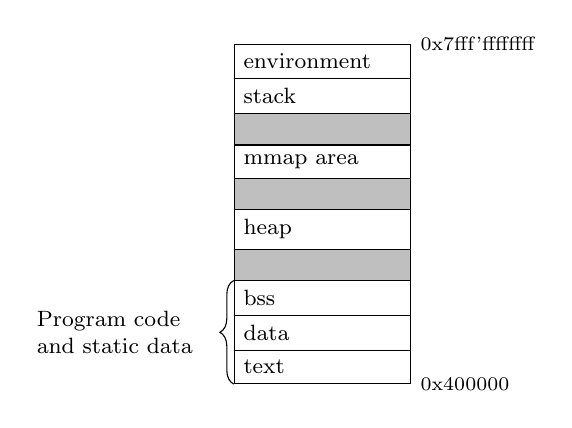
\begin{tikzpicture}[font=\footnotesize]

    % See page 453 in pgf manual
    \node [
      rectangle split, rectangle split parts=10, 
      rectangle split part fill={white, white, lightgray, white, lightgray, white, lightgray, white},
      draw, anchor=center, text width=2cm
    ] (m)
      {
        \nodepart{one}
          environment
        \nodepart{two}
          stack
        \nodepart{four}
          mmap area
        \nodepart{six}
          heap
        \nodepart{eight}
          bss
        \nodepart{nine}
          data
        \nodepart{ten}
          text
      };

    \draw [decorate, decoration={brace, amplitude=5pt}] (m.south west) -- (m.seven split west) 
      node [black, midway, xshift=-1.5cm, text width=2.0cm] 
        { Program code and static data } ;

    \node[right] at (m.north east)
      { \scriptsize{0x7fff'ffffffff} } ;

    \node[right] at (m.south east)
      { \scriptsize{0x400000} } ;

  \end{tikzpicture}
\end{figure}

Text and data sections contain program code and static data respectively.
These regions are mapped towards the low en of the address spectrum, and the virtual addresses of variables allocated here will not change with environment size. 

Note that the initial position of stack will not depend on environment size this way when address randomization (ASLR) is enabled. (TODO: Does it offset from page boundary? That would be good, same alias behavior :)

Addresses of stack allocated variables can vary depending on environment size, while other segments of memory such as text and data remain constant over all environments.

To illustrate how this can cause bias, we revisit the example first presented in~\cite{Mytkowicz:2009:WrongData}, shown in Listing~\ref{lst:loopkernel}. 
This example is interesting for several reasons. 
The bias effects are significant and easily reproducible, while the example code is simple and easy to analyze.
Still, no satisfactory explanation as to what causes bias was given in the original paper.

\begin{lstlisting}[float=h, language=C, caption={Microkernel succeptible to aliasing between static variables and automatic variables for certain environment sizes}, label={lst:loopkernel}, frame=lines]
static int i, j, k;
int main() {
    int g = 0, inc = 1;
    for (; g < 65536; g++) {
        i += inc;
        j += inc;
        k += inc; 
    }
    return 0;
}
\end{lstlisting}

Their program contains five variables, two of which are stack allocated and i, j and k that are statically allocated.
Performance counter measurements of cycle counts are shown for 512 different environment sizes in Figure~\ref{fig:envbias}.
Sampling is done for every 16 byte increment of environment size, covering two 4K periods of addresses.
A finer sampling is not necessary, because the stack is by default aligned to 16 byte.
The program is compiled with GCC using no optimization.
Any optimization would likely disregard most of the function as redundant code, and reduce it to return zero immediately.

There are clearly two worst cases, indicated by significant spikes around the 3100 and 7100 byte offsets.
We analyzed these cases by sampling an extensive set of performance counters and correlating them with cycle counts.
The results show a high number of resource stalls when the spikes occur, indicated by high values for performance counters \small{RESOURCE\_STALLS.ANY}, \small{CYCLE\_ACTIVITY.CYCLES\_LDM\_PENDING}, \small{CYCLE\_ACTIVITY.CYCLE\_NO\_EXECUTE} and \small{RESOURCE\_STALLS.RS}.
We also find that \small{LD\_BLOCKS\_PARTIAL.ADDRESS\_ALIAS} correlates almost perfectly with cycle count, which can explain the high number of resource stalls with false dependency from aliasing.

\subsection{Finding Collisions}
To be able to explain what is happening in this case we need to know the addresses of all variables at run time.
For statically allocated data, memory allocation is decided at compile time.
The location of variables i, j and k can be found by looking at the symbol table in the ELF executable.
Below is an excerpt of \lstinline$readelf -s$.
\begin{lstlisting}[float=h, basicstyle=\small]
37: 000000000060103c    4  (...)  25 i
38: 0000000000601040    4  (...)  25 j
39: 0000000000601044    4  (...)  25 k
\end{lstlisting}

Need to observe run time addresses without introducing any observer effects.
A small amount of assembly code was used to calculate the addresses of each stack allocated variable and output them directly using system calls, without impacting run time addresses.
We find that the spike in cycle count occurs when the address of inc alias with i, where the first spike happens when inc is at 0x7fffffffe03c.
Because the stack is aligned to 16 byte or 4 words, there are a couple of different scenarios that could have been observed here.
Static area is fixed and covers 12 contiguous bytes (3 words) \lstinline$[x|x| |x]$.
Automatic variables occupies 8 contiguous bytes on stack (2 words) [ | |x|x]. 
The space of possible addresses for (inc, g) in this case is (0x7fffffffe03c, 0x7fffffffe038) - n*4096. 
In this scenario, g will never alias with any of the static variables -- as it always covers the 0x8 slot not occupied by either of i, j or k.
An even worse case with respect to the number of alias events is if allocation of static data allows collisions with both stack allocated variables.
This can be achieved by reserving an extra 8 bytes to offset i, j into the 0x8, 0xc slots. 
While this will give significantly more alias counts, it has little effect on the number of cycles executed.

Worst case occurs for precisely one out of 256 possible initial stack addresses in every 4K segment.
Resource stalls are generated because of false dependencies between stack and static data, resulting in worse performance.
The program is \emph{biased} towards environment sizes that avoids this specific stack alignment.


\subsection{Avoiding Aliasing}
Addresses of automatic variables can not be determined statically, because the position of stack at runtime is generally unknown. 
In addition to being offset by environment variables, the stack address can also be perturbed by other factors such as address layout randomization. 
Although one can not easily know if a collision is going to happen for a given environment, one can try to change the program to account for possible alias effects.
The following strategy is a proof of concept of how alias-free code can be generated in this particular case.
If the addresses do alias, branch to an alternative but semantically equivalent code path.
Allocate a new set of variables to avoid aliasing.

\begin{lstlisting}[float=h, language=C, caption={Dynamically detect aliasing case, and avoid by pushing another stack frame.}, label={lst:loopfixed}, frame=lines]
#define ALIAS(a, b) \
    ((((long)&a)&0xfff)==(((long)&b)&0xfff))
static int i, j, k;
int main() {
    int g = 0, inc = 1;
    if (ALIAS(inc, i) || ALIAS(g, i))
        return main();
    for (; g < 65536*10; g++) {
        i += inc;
        j += inc;
        k += inc;
    }
    return 0;
}
\end{lstlisting}



\section{Bias from Heap Allocation}
Address aliasing can be caused by conflicting pairs of load/store operations to any part of memory.
The previous section looked specifically at an example of collision between stack variables and static data.
Another scenario to consider is collisions in heap allocated memory.
In particular, code that operate on pairs of contiguous arrays can be vulnerable to 4K aliasing.
Acquiring dynamic memory at run time is usually done by calling malloc, which takes a number of bytes to allocate and returns a pointer to that area.
A typical malloc implementation uses two different strategies for how to allocate memory.
The \emph{heap} area in virtual memory is used for smaller allocations.
Programs are initially given a small heap area, which the allocator can increase by calling brk or sbrk.
For larger allocations, it is typically faster to use anonymous memory mapping by calling mmap, instead of growing the ``normal'' heap.
The heap starts at a low address close to the data section and grows towards higher addresses. 
Mmap allocates much closer to the stack.
While heap addresses can look like 0x16e30a0 or 0x1723020, pointers returned by mmap can for example be 0x7f0318a8f010 or 0x7f03105d2010.
This distinction is of course unimportant for application developers, as everything is conceptually the same ``heap''.
However, mmap has an interesting property in that allocations will always be page aligned.
The page size is 4096 bytes, meaning two pointers returned by mmap will \emph{always} alias.\footnote{libc's version of malloc adds 16 bytes of medatada at the beginning, therefore every mmap'ed address ends with 0x010}

\subsection{Aligned Sequential Access}
Consider the function shown in Listing~\ref{lst:conv}.
It computes the convolution between an input array and a fixed five-element kernel, writing the result to another array.
For simplicity, endpoints are not handled.

\pgfplotstableread{bin/convolution.dat}{\convolutiontable}
\begin{figure}[t]
  \caption{Cycle and alias counts for different offsets between input and output arrays in Listing~\ref{lst:conv}. Offset 0 means equal 12 bit address suffix, which is default behavior for mmap allocations. Array size $n=2^{20}$, compiled with -O3. }
  \label{fig:heapalias}
  \begin{tikzpicture}
    \begin{axis}[
        font = \small,
        xlabel=Relative offset in \lstinline!sizeof(float)! bytes,
        cycle list name=black white
      ]
      \addplot table[x expr = \thisrowno{0}, y = cycles:u] \convolutiontable ;
      \addplot table[x expr = \thisrowno{0}, y = r0107:u ] \convolutiontable ;
      \addlegendentry{cycles:u} ;
      \addlegendentry{r0107:u} ;
    \end{axis}
  \end{tikzpicture}
\end{figure}

\begin{lstlisting}[float=h, language=C, caption={Naive implementation of convolution. Highly sensitive to aliasing between input and output arrays.}, label={lst:conv}, frame=lines]
static float k[5]={0.1,0.25,0.3,0.25,0.1};
void conv(int n, float *in, float *out) {
    int i, j;
    for (i = 2; i < n-2; ++i) {
      out[i] = 0;
      for (j = 0; j < 5; ++j)
          out[i] += in[i-2+j] * k[j];
    }
}
\end{lstlisting}

Figure \ref{fig:heapalias} shows how this function behaves when given input with different alignment.
The default behavior for large heap allocations is that both arrays alias.
To force different alignments, we allocate some extra bytes at the end and offset the output pointer argument.

\begin{lstlisting}
output = malloc(n * (sizeof(float) + offset));
conv(n, input, output + offset);
\end{lstlisting}

Listing \ref{lst:conv}, together with a small main method handling the allocation and offset, is compiled with optimization O3 and input size n=$2^{20}$.
Figure \ref{fig:heapalias} plots performance counter statistics for cycle count and 4K alias events over increasing amount of offset.
This is an example of how false dependencies from address aliasing can cause a significant performance hit.
Because large heap allocations always alias, the processor thinks memory accesses to input[i] potentially conflicts with output[i], stalling the pipeline.
By manually adjusting the alignment of one input buffer, cycle count can be reduced by more than 50\% (verify).
This is a speedup on top of compiler optimization O3, which is not able to account for aliasing effects.

It is perhaps unfair to assume the compiler can fix this when only given a generic optimization flag, as aliasing effects is (presumably) an Intel-specific issue.
You might also want to utilize the C99 keyword restrict to explicitly tell the compiler that the buffers are disjoint in memory.

\begin{lstlisting}[language=C]
void conv( int n,
            const float * restrict in,
            const float * restrict out );
\end{lstlisting}

Even with the updated signature compiled with -O3 -march=native, there is still room for improvement by inserting manual offsets.


\subsection{Behavior of other Allocators}
As with the contents of environment variables, the exact behavior of dynamic memory allocation can typically not be known ahead of time.
Heap allocation routines such as malloc and free are usually dynamically linked and resolved at run-time, which again represents a source of potential bias.
For the code examples presented earlier, the dynamic linker will resolve malloc to some version of glibc, which is the default on our system.
Variations between different versions of libc, or local configurations on parameters such as M\_MMAP\_THRESHOLD, could trigger aliasing cases.

In addition to glibc's ptmalloc, we look at the following alternatives.
\begin{itemize}
 \item Thread-Caching Malloc (ptmalloc) is developed by Google. It aims to be time and space efficient, and reduces lock contention for multithreaded applications. \cite{TCMalloc}
 \item jemalloc was originally developed for FreeBSD. It aims to be a scalable general purpose allocator in single or multithreaded environments. \cite{JEMalloc}
 \item Hoard is another project that focuses extensively on improving performance for multithreaded programs. \cite{Berger:2000:Hoard}
\end{itemize}

\begin{table}[t]
  \caption{Addresses returned by different heap allocators when allocating pairs of equally sized buffers}
  \label{tab:mallocompare}
  \centering
  \small
  \begin{tabular}{l r r}
    \toprule
                      & 5120 B          & $2^{20}$ B \\
    \midrule
    glibc             & 0x6028d0        & 0x2aaaaaaf3010 \\
    (ptmalloc)        & 0x603ce0        & 0x2aaaab098010 \\
    \midrule
    tcmalloc          & 0xe16000        & 0xe64000 \\
                      & 0xe18800        & 0xf64000 \\
    \midrule
    jemalloc          & 0x2aaaabc1f000  & 0x2aaaabc86000 \\
                      & 0x2aaaabc21000  & 0x2aaaabd86000 \\
    \midrule
    Hoard             & 0x2aaaaab40070  & 0x2aaaabf40070 \\
                      & 0x2aaaaab42070  & 0x2aaaac060070 \\
    \bottomrule
  \end{tabular}
\end{table}

Table \ref{tab:mallocompare} illustrates some differences that can be observed by switching heap allocator. \footnote{Switching allocator was done by setting the LD\_PRELOAD environment variable.}
The addresses of two equally sized char buffers allocated with malloc are observed for size parameters 5120 and $2^{20}$ bytes. 
We do not care about performance, only the actual memory addresses returned and whether they alias or not.

For smaller allocations, we see that glibc and tcmalloc uses the normal heap area -- returning numerically low addresses.
Interestingly, jemalloc and Hoard appears to never use brk, but always allocate to mmaped areas even for smaller sizes.
We see one example where one allocator yields aliasing buffers while another does not. 
Allocating $2 \times 5120 B$ returns aliasing pointers for jemalloc and Hoard, but not with glibc or tcmalloc.
Given that these results are deterministic (with ASLR disabled), it is not hard to construct a program with significant bias towards one or the other allocator.

Most malloc alternatives focuses heavily on performance in multithreaded environments.
Heap allocation is intrinsically inefficient in that all threads share the same address space, leading to a high potential lock contention on memory accesses.
To our knowledge, there are no commonly used allocators that specifically tries to mitigate aliasing in heap allocated memory.
This dispite explicit recommendation from Intel that special purpose allocators should care about aliasing for optimization. [cite]

The purpose of this is to illustrate that allocators is yet another source of bias.
Using heap allocated memory, address aliasing is an artifact of the allocator used.
With different versions or configurations of memory allocators, any performance impact from aliasing can qualify as measurement bias.


\iffalse

\section{Optimizing Alignment in BLAS}

To illustrate how real world applications can be impacted by aliasing, we look at low level numerical applications.
In this section we show that even highly optimized numerical libraries suffer performance degradation from aliasing.
Basic Linear Algebra Subroutines (BLAS), is the de facto standard API for high performance linear algebra routines.
The functionality is divided into three categories: 

\begin{description}
  \item{Level~1} Scalar and vector operations, such as dot product and vector addition.
  \item{Level~2} Matrix-vector operations, such as gemv for general matrix-vector multiplication.
  \item{Level~3} Matrix-matrix operations, including the widely applied gemm routine for general matrix-matrix multiplication. 
\end{description}

Functions operating on vectors, from BLAS Level 1 or 2, intuitively appears the most likely to have potential for aliasing.
Many highly optimized implementations of BLAS exists, ATLAS being a widely used and open source alternative. One of the key features of ATLAS is that it uses automatic tuning to optimize for cache efficiency [Whaley:2000:ATLAS]. 

We use the currently latest stable version 3.10.1 of ATLAS, built as a shared library from source.
The automatic tuning happens during the build process; A series of test programs are run to determine cache edges and other properties of the hardware, which in turn affects the resulting binary. 

Carefully monitoring cache metrics is particularly important in this case study, as BLAS performance heavily relies on cache efficiency.
Relevant performance statistics for cache hit ratios was considered to rule out cache as the cause of any bias effects.
In addition, we disable hardware prefetching in BIOS to further minimize cache impacts. 
Note however that the same conclusions can be drawn independently of these measures.

\subsection{Aliasing in cblas\_daxpy}
Found aliasing here as well. Two spikes, not sure why. Might want to test other BLAS libraries. Include or leave out? Too much handwaving and too little analysis maybe. Depends on the target paper length as well?



\subsection{Matrix vector multiplication}

Consider matrix-vector multiplication of the form $\boldsymbol{y} = A\boldsymbol{x} + \boldsymbol{b}$.
Let A be of size $M \times N$, where M is the number of rows. 

$
\left[\begin{array}{ccccc}
a_{0,0} & a_{0,1} &  &  & a_{0,N}\\
a_{1,0}\\
 &  &  & \ddots\\
a_{M,0} &  &  &  & a_{M,N}
\end{array}\right]\left[\begin{array}{c}
x_{0}\\
x_{1}\\
\vdots\\
\\
x_{N}
\end{array}\right]=\left[\begin{array}{c}
y_{0}\\
y_{1}\\
\vdots\\
y_{M}
\end{array}\right]
$

General matrix vector multiplication is implemented by the level 2 gemv routine, computing $\boldsymbol{y} = \alpha\text{op}\left(A\right)\boldsymbol{x} + \beta\boldsymbol{y}$
Here, $\alpha$ and $\beta$ are constants, and $\text{op}\left(A\right)$ is an optional transpose or complex conjugate of the matrix. 
We set $\alpha = 1$, $\beta = 0$ and $\text{op} \left(A\right) = A$ to reduce the formula to $\boldsymbol{y}=A\boldsymbol{x}$.
[There are three memory buffers involved, and one might suspect that implementations are succeptible to aliasing between of $\boldsymbol{A}$, $\boldsymbol{x}$ or $\boldsymbol{y}$.]
For the following discussion we look at a particular configuration where $A$ is of size $64\times64$.

In order to accurately measure any effects of aliasing, we need to isolate the actual function call from heap allocation and initialization code.
This is done by running the program twice for each memory configuration, one where cblas\_dgemv is executed $K = 101$ times in a tight loop.
An approximation of the cost for a single function invocation can be expressed as 
$$
t_{\text{estimate}}=\frac{t_{K=101}-t_{K=1}}{100}
$$
where t represents some metric, such as the number of cycles.
Subtracting the $K = 1$ run removes the constant overhead from the $K = 101$ run, and dividing by $100$ averages the values from the remaining iterations.
Other iteration counts could have been used as well.

Figure \ref{fig:heatmap} shows estimated number of alias events for every relevant memory configuration possible for cblas\_dgemv with matrix size 64 $\times$ 64. 
While matrix A is kept fixed at address suffix 0x000, every reasonable variation of (\&x, \&y) is measured.
Each increment represents an address offset of 16 bytes, which is the same granularity one would get from the default heap allocator.
In a 4K address space, there are thus $4096/16 = 256$ possible address suffixes for $\boldsymbol{x}$ and $\boldsymbol{y}$ independently, resulting in a grid of $256^2$ values.

\begin{figure}[h]
  \caption{Estimated aliasing cost of invoking cblas\_dgemv with a matrix size $64 \times 64$ for different memory layouts. Axis show address offsets times 0x10 for vectors $\boldsymbol{x}$ and $\boldsymbol{y}$. Matrix $A$ has fixed to address suffix 0x000.}
  \label{fig:heatmap}
  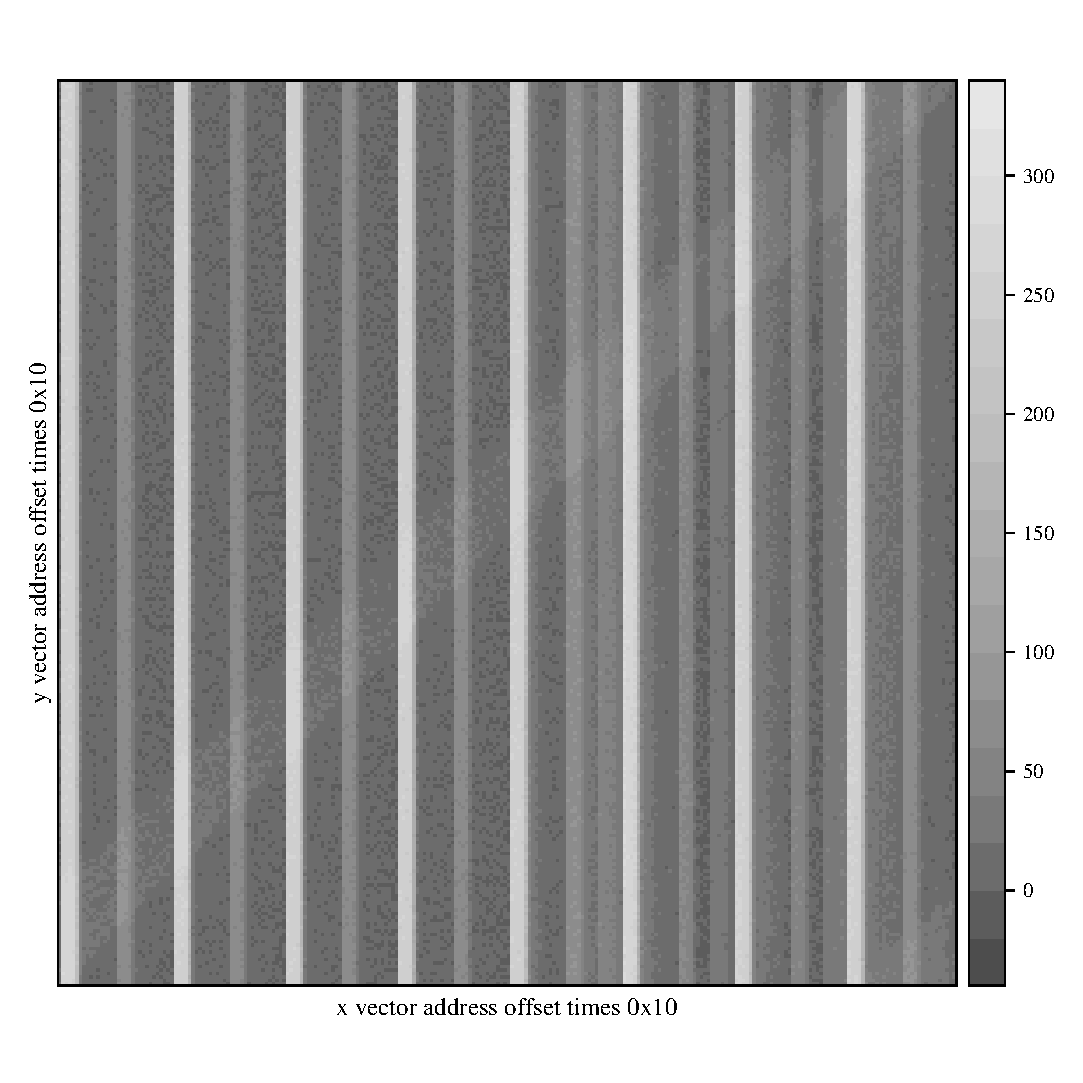
\includegraphics[width=\columnwidth]{resources/heatmap.eps}
\end{figure}

It appears that aliasing is mostly dependent on the location of $\boldsymbol{y}$, in this case with 8 distinct worst case regions.
This is consistent with false dependencies between $\boldsymbol{y}$ and specific rows in A. 
The first bad region is where $\&y ~= 0$, matching the first row of A. 



\begin{table*}[t]
  \caption{Estimated cost of invoking cblas\_dgemv with a matrix size $8192 \times 8192$}
  \label{tab:atlas8k}
  \small
  \centering
  \begin{tabular}{l r r r}
    \toprule
      & (0x010, 0x010, 0x020) & (0x010, 0x010, 0x0b0) & (0x010, 0x140, 0x150) \\
    \midrule
    \perfctr{cpu_clk_unhalted.thread_p} & 162,926,895 & 152,151,263 & 144,583,160 \\
    \perfctr{ld_blocs_partial.address_alias} & \textbf{68,408,790} & \textbf{5,154,981} & \textbf{2,919} \\

    \perfctr{mem_uops_retired.all.loads} & 100,701,777 & 100,702,138 & 100,701,752 \\
    \perfctr{mem_load_uops_retired.hit_lfb} & 31,628,539 & 32,495,287 & 29,853,850 \\
    \perfctr{mem_load_uops_retired.l1_hit} & 68,309,447 & 65,625,881 & 69,387,368 \\
    \perfctr{mem_load_uops_retired.l2_hit} & 711,973 & 1,540,956 & 864,720 \\
    \perfctr{mem_load_uops_retired.l3_hit} & 154,345 & 651,985 & 363,331 \\
    \perfctr{mem_load_uops_retired.l3_miss} & 106,313 & 350,449 & 295,235 \\
    \perfctr{mem_load_uops_retired.all_stores} & 33,562,692 & 33,562,692 & 33,562,692 \\

    \perfctr{load_hit_pre.hw_pf} & 42,914,191 & 47,315,935 & 59,211,320 \\
    \bottomrule
  \end{tabular}
\end{table*}

Notes: 
 - More BR\_INST.COND.TAKEN taken in case (a), but number of retired instructions are the same. Suggests replays of instructions.
 - Inverse HW prefetch numbers from masters

\paragraph{Prefetching}
Measurements repeated with prefetching disabled, giving similar results. 

Estimated performance counter statistics for each of the three heap address configurations are shown in Table [?tab:gemv-estimate].
In addition to cycle count and alias events, a number of relevant metrics related to cache activity are also included.
Notice that almost all load micro-ops are served by either the line fill buffer or L1 cache in all cases.
Only a small amount of loads come from L2, and almost none from L3.
The hit rate for L1 actually decreases somewhat (considering LFB as well) with better execution time.
This could be explained by less time for prefetchers to feed the L1 cache with data.
The hardware prefetch counter indicates more hits in cases a and b.
Again, we find that cache efficiency does not explain the performance cliffs we observe. 

Our results show that address aliasing between matrix and vector heap buffers can significantly impact performance of dgemv in ATLAS.
Variations in heap addresses alone can give a speedup of more than 30 \%.


\subsection{Dealing with Aliasing}
For the particular case we investigated, a good heuristic is to align heap segments “far apart” within the 4 KiB area of 12 bit suffixes.
More specifically, it appears that address suffixes of A and $\boldsymbol{y}$ are the most important to separate.

As discussed in section [x], aliasing cases like these can be accounted for in software using padding techniques.
A possible run time solution to adjust heap addresses can be realized as follows:

\begin{itemize}
  \item Allocate some extra space for one of the vectors when calling malloc, for instance sizeof(double) * (M + 0x100) for $\boldsymbol{y}$.

  \item Check the returned pointers for potential alias, i.e. the difference between \&A and \&y. Offset using pointer arithmetic into the array with extra padding at the end, i.e. y += 0x100. 
\end{itemize}

Another option is to explicitly account for “worst cases” in the implementation of routines that are vulnerable to aliasing.
Addresses can be explicitly checked for potential conflicts in cblas\_dgemv, and if possible branch to code that will not suffer from aliasing. 

\fi


\section{Conclusions}
In this paper we have looked at how address aliasing can affect program performance under different memory layouts, and how it can explain certain cases of measurement bias. 
The effect is caused by the way speculative and out-of-order memory operations are handled by the CPU, only considering the last 12 address bits to resolve conflicts load and store operations.

Analyzing the example originally presented by Mytkowicz et al. \cite{Mytkowicz:2009:WrongData}, we determined that collisions between stack variables and static data resulted in aliasing for certain stack positions.
In this case, the external trigger of bias is variations in environment size, which in turn offset the virtual addresses of stack allocated variables.


In general, any change to virtual memory layout of data can potentially introduce bias effects from address aliasing. 
We present a code example with extreme sensitivity of data alignment, with more than 50 \% performance variation between different memory layouts.


We find that compilers, even when provided with architecture specific optimization flags, still generates code that suffers from aliasing. 
Typical heap allocators return page-aligned memory by default, which is the worst case with respect to aliasing for many algorithms.
Despite recommendations from Intel, we are not aware of any allocators that specifically addresses this issue. 
We show how manual padding of variables, and alternative alias-free code paths, can be used to avoid aliasing at run time.
This means that an understanding of 4K address aliasing is sometimes needed to achieve optimal performance. 


%\onecolumn

\bibliographystyle{plain}
\bibliography{references}

\end{document}
